%%%%%%%%%%%%%%%%%%%%%%%%%%%%%%%%%%%%%%%%%%%%%%%%%%%%%%%%%%%%%%%%
%  文章模板:A4 纸,小五字,单列(可根据要求改双列 twocolumn)
%%%%%%%%%%%%%%%%%%%%%%%%%%%%%%%%%%%%%%%%%%%%%%%%%%%%%%%%%%%%%%%%
\documentclass[a4paper,11pt,onecolumn,twoside]{article}

%%%%%%%%%%%%%%%%%%%%%%%%%%%%%%%%%%%%%%%%%%%%%%%%%%%%%%%%%%%%%%%%
%  packages
%    这部分声明需要用到的包
%%%%%%%%%%%%%%%%%%%%%%%%%%%%%%%%%%%%%%%%%%%%%%%%%%%%%%%%%%%%%%%%
\usepackage{CJK}         % CJK 中文支持
\usepackage{fancyhdr}
\usepackage{amsmath,amsfonts,amssymb,graphicx}    % EPS 图片支持
\usepackage{subfigure}   % 使用子图形
\usepackage{indentfirst} % 中文段落首行缩进
\usepackage{bm}          % 公式中的粗体字符(用命令\boldsymbol)
\usepackage{multicol}    % 正文双栏
\usepackage{indentfirst} % 中文首段缩进
\usepackage{picins}      % 图片嵌入段落宏包 比如照片
\usepackage{abstract}    % 2栏文档,一栏摘要及关键字宏包
\usepackage[ruled]{algorithm2e} 
\usepackage{enumerate}
\usepackage{enumitem}

%%%%%%%%%%%%%%%%%%%%%%%%%%%%%%%%%%%%%%%%%%%%%%%%%%%%%%%%%%%%%%%%
%  lengths
%    下面的命令重定义页面边距,使其符合中文刊物习惯。
%%%%%%%%%%%%%%%%%%%%%%%%%%%%%%%%%%%%%%%%%%%%%%%%%%%%%%%%%%%%%%%%
\addtolength{\topmargin}{-54pt}
\setlength{\oddsidemargin}{-0.9cm}  % 3.17cm - 1 inch
\setlength{\evensidemargin}{\oddsidemargin}
\setlength{\textwidth}{17.00cm}
\setlength{\textheight}{24.00cm}    % 24.62

%%%%%%%%%%%%%%%%%%%%%%%%%%%%%%%%%%%%%%%%%%%%%%%%%%%%%%%%%%%%%%%%
%  定义标题格式,包括title,author,affiliation,email等。
%  在任何用到中文的地方,用\begin{CJK} ... \end{CJK}将其括起来。
%%%%%%%%%%%%%%%%%%%%%%%%%%%%%%%%%%%%%%%%%%%%%%%%%%%%%%%%%%%%%%%%

\renewcommand{\baselinestretch}{1.1} %定义行间距
\parindent 22pt %重新定义缩进长度

%%%%%%%%%%%%%%%%%%%%%%%%%%%%%%%%%%%%%%%%%%%%%%%%%%%%%%%%%%%%%%%%
% 标题,作者,通信地址定义
%%%%%%%%%%%%%%%%%%%%%%%%%%%%%%%%%%%%%%%%%%%%%%%%%%%%%%%%%%%%%%%%
\begin{CJK}{GBK}{song}
\title{\huge{差分进化算法简介}}
\author{张甲栋 \\[2pt]
\normalsize
(浙江大学计算机科学与技术学院,浙江省~杭州市~310000) \\[2pt]}
\date{}  % 这一行用来去掉默认的日期显示
\end{CJK}

%%%%%%%%%%%%%%%%%%%%%%%%%%%%%%%%%%%%%%%%%%%%%%%%%%%%%%%%%%%%%%%%
% 首页页眉页脚定义
%%%%%%%%%%%%%%%%%%%%%%%%%%%%%%%%%%%%%%%%%%%%%%%%%%%%%%%%%%%%%%%%
\fancypagestyle{plain}{
\fancyhf{}
\chead{\centering{生~~物~~智~~能~~算~~法}}
\lfoot{}
\cfoot{}
\rfoot{}}

%%%%%%%%%%%%%%%%%%%%%%%%%%%%%%%%%%%%%%%%%%%%%%%%%%%%%%%%%%%%%%%%
% 首页后根据奇偶页不同设置页眉页脚
% R,C,L分别代表左中右,O,E代表奇偶页
%%%%%%%%%%%%%%%%%%%%%%%%%%%%%%%%%%%%%%%%%%%%%%%%%%%%%%%%%%%%%%%%
\pagestyle{fancy}
\fancyhf{}
\fancyhead[CE,CO]{生~~物~~智~~能~~算~~法}
\fancyhead[RE,RO]{\thepage}
\lfoot{}
\cfoot{}
\rfoot{}

%%%%%%%%%%%%%%%%%%%%%%%%%%%%%%%%%%%%%%%%%%%%%%%%%%%%%%%%%%%%%%%%
% 正文两栏环境不允许float环境,比如 figure, table。所以重新定义
% figure,使之可以浮动到你想要的位置。table也同样,把figure改为
% table就可以。
%%%%%%%%%%%%%%%%%%%%%%%%%%%%%%%%%%%%%%%%%%%%%%%%%%%%%%%%%%%%%%%%
\newenvironment{figurehere}
  {\def\@captype{figure}}
  {}
\makeatother


%%%%%%%%%%%%%%%%%%%%%%%%%%%%%%%%%%%%%%%%%%%%%%%%%%%%%%%%%%%%%%%%
%  文章正文
%%%%%%%%%%%%%%%%%%%%%%%%%%%%%%%%%%%%%%%%%%%%%%%%%%%%%%%%%%%%%%%%
\begin{document}
\begin{CJK*}{GBK}{song}
\CJKcaption{GB}

%%%%%%%%%%%%%%%%%%%%%%%%%%%%%%%%%%%%%%%%%%%%%%%%%%%%%%%%%%%%%%%%
%  自定义命令
%%%%%%%%%%%%%%%%%%%%%%%%%%%%%%%%%%%%%%%%%%%%%%%%%%%%%%%%%%%%%%%%
% 此行使文献引用以上标形式显示
\newcommand{\supercite}[1]{\textsuperscript{\cite{#1}}}

%%%%%%%%%%%%%%%%%%%%%%%%%%%%%%%%%%%%%%%%%%%%%%%%%%%%%%%%%%%%%%%%
%  显示title,并设页码为空(按杂志社要求)
%%%%%%%%%%%%%%%%%%%%%%%%%%%%%%%%%%%%%%%%%%%%%%%%%%%%%%%%%%%%%%%%
\maketitle

%%%%%%%%%%%%%%%%%%%%%%%%%%%%%%%%%%%%%%%%%%%%%%%%%%%%%%%%%%%%%%%%
%%%%%%%%%%%%%%%%%%%%%%%%%%%%%%%%%%%%%%%%%%%%%%%%%%%%%%%%%%%%%%%%
%  中文摘要
%  调整摘要、关键词,中图分类号的页边距
%  中英文同时调整
%%%%%%%%%%%%%%%%%%%%%%%%%%%%%%%%%%%%%%%%%%%%%%%%%%%%%%%%%%%%%%%%
\setlength{\oddsidemargin}{ 1cm}  % 3.17cm - 1 inch
\setlength{\evensidemargin}{\oddsidemargin}
\setlength{\textwidth}{13.50cm}
\vspace{-.8cm}
\begin{center}
\parbox{\textwidth}{
\CJKfamily{hei}摘~~~要\quad \CJKfamily{kai}~差分进化算法(DE)是一类基于种群的启发式全局搜索技术,
具有全局优化性能好、结构简单和易于实现等优点。本文围绕差分进化算法的原理、特点、改进以及应用等
方面,对差分进化算法进行了详细的介绍,在此基础上,对差分进化算法的进一步发展进行了探讨和展望。\\
\CJKfamily{hei}关键词\quad\CJKfamily{kai}差分进化,进化算法,启发式搜索}
\end{center}

%%%%%%%%%%%%%%%%%%%%%%%%%%%%%%%%%%%%%%%%%%%%%%%%%%%%%%%%%%%%%%%%
%  英文摘要
%%%%%%%%%%%%%%%%%%%%%%%%%%%%%%%%%%%%%%%%%%%%%%%%%%%%%%%%%%%%%%%%
\vspace{.1cm}
\begin{center}
\parbox{\textwidth}{
{\large{\textbf{A brief introduction of Differential Evolution Algorithm}}}\\
\vspace{-0.5cm}
\begin{center}
\textbf{Zhang Jiadong}\\[2pt]
\small{\textit{(College of computer science and technology, Zhejiang University, Hangzhou, 310000)}}\\[2pt]
\end{center}
{\small{\textbf{Abstract}\quad Differential Evolution Algorithm(DE) is a kind of heuristic global search 
technology based on population. It has the advantages of good global optimization performance , simple 
structure and easy to implement. In this paper, the Differential Evolution Algorithm is introduced in detail 
based on the principles, characteristics, improvements and applications of this algorithm. Finally, the further 
development of Differential Evolution Algorithm is discussed and prospected. \\
\textbf{Key Words}\quad Differential Evolution, Evolutionary Algorithms, Heuristically Search}}
}
\end{center}


%%%%%%%%%%%%%%%%%%%%%%%%%%%%%%%%%%%%%%%%%%%%%%%%%%%%%%%%%%%%%%%%
%  正文由此开始-------------------------
%%%%%%%%%%%%%%%%%%%%%%%%%%%%%%%%%%%%%%%%%%%%%%%%%%%%%%%%%%%%%%%%
%%%%%%%%%%%%%%%%%%%%%%%%%%%%%%%%%%%%%%%%%%%%%%%%%%%%%%%%%%%%%%%%
%  恢复正文页边距
%%%%%%%%%%%%%%%%%%%%%%%%%%%%%%%%%%%%%%%%%%%%%%%%%%%%%%%%%%%%%%%%
\setlength{\oddsidemargin}{-.5cm}  % 3.17cm - 1 inch
\setlength{\evensidemargin}{\oddsidemargin}
\setlength{\textwidth}{17.00cm}
\CJKfamily{song}

%%%%%%%%%%%%%%%%%%%%%%%%%%%%%%%%%%%%%%%%%%%%%%%%%%%%%%%%%%%%%%%%
%  分栏开始
\begin{multicols}{2}
%%%%%%%%%%%%%%%%%%%%%%%%%%%%%%%%%%%%%%%%%%%%%%%%%%%%%%%%%%%%%%%%
\section{引言}
%%%%%%%%%%%%%%%%%%%%%%%%%%%%%%%%%%%%%%%%%%%%%%%%%%%%%%%%%%%%%%%%
%  调整section名称与正文之间的距离
%%%%%%%%%%%%%%%%%%%%%%%%%%%%%%%%%%%%%%%%%%%%%%%%%%%%%%%%%%%%%%%%
\indent 差分进化算法(Differential Evolution, DE)\supercite{1,2}是一种基于群体智能的全局优化方法。
它由Storn等人于1995年提出,最初用于求解切比雪夫多项式问题,后来也被用于解决复杂的优化问题。
差分进化算法属于进化算法(evolutionary algorithms, EAS)的一种。相比于传统的进化算法,差分进化算法
采用基于差分的简单变异操作和一对一的生存竞争策略,降低了遗传操作的复杂性。另外,差分进化算法可以
动态调整搜索策略,具有较强的全局搜索能力以及鲁棒性,适于求解常规数学方法无法求解的全局优化问题。\\
\indent 目前,差分进化算法已在很多领域得到了应用。在人工神经网络领域,Liu等\supercite{3}将差分
进化算法与混沌搜索相结合来训练多层前馈神经网络。在化工领域,Kiranmai等\supercite{4}利用差分进化
算法确定固定薄膜生物反应的机理参数。在机器人领域,Aydin等\supercite{5}将差分进化算法与模糊推理
相结合,用于解决机器人最优路径规划问题。此外,差分进化算法在电力系统、机械设计、信号处理、生物学、
运筹学等领域也有广泛的应用。本文首先对标准的差分进化算法进行介绍,在此基础上,提出差分进化算法的
改进策略,进一步将基本进化算法与差分进化算法进行比较。最后,对全文进行总结,对差分进化算法的发展
进行展望。

\section{算法介绍}
\subsection{标准差分进化算法}
\indent 差分进化算法本质是一种基于实数编码的具有保优思想的贪婪遗传算法\supercite{6}。它通过种群
之间的个体差异和优胜劣汰的竞争策略产生新的个体,最终使种群接近或达到全局最优解。差分进化算法伪码
描述如算法1所示。首先在问题的可行解空间随机初始化种群$X^0=[x_1^0,x_2^0,...,x_M^0]$, $M$为初始种群
的规模。个体$x_i^0=[x_{i,1}^0,x_{i,2}^0,...,x_{i,D}^0]$表征问题解,$D$为问题解空间的维数。然后,
对初始种群进行变异和交叉操作,产生新的种群。针对原种群和新种群中的个体,采用贪心思想,进行一对一的选择,
作为下一代种群。通过不断迭代,标准差分进化算法使种群向着问题最优解方向进化,从而不断逼近问题的最优解。
当达到一定的误差要求或迭代次数超过设定值时,算法停止,此时种群中的最优个体即为算法求得的问题解。\\

\begin{algorithm}[H]  
\caption{Differential Evolution algorithm}  
\KwIn{Population: $M$; Dimension: $D$; Genetation: $T$}  
\KwOut{The best vector(solution): $\Delta$}  
initialization\;
\For{$i=1$ to $M$}
{
	\For{$j=1$ to $D$}
	{
		$x_{i,j}^t=x_{min,j}^t+rand(0,1)*(x_{max,j},-x_{min,j})$\
	}
}
\While{$|f(\Delta)|>\varepsilon$ or $t<T$}{  
    \For{$i=1$ to $M$}
	{
		Mutation and Crossover\;
		\For{$j=1$ to $D$}
		{
			$v_{i,j}^t=Mutation(x_{i,j}^t)$\;
			$u_{i,j}^t=Crossover(x_{i,j}^t,v_{i,j}^t)$\;
		}
		Greedy Selection\;
		\eIf{$f(u_{i}^t)<f(x_{i}^t)$}
		{
			$x_{i}^t\leftarrow u_{i}^t$\;
			\If{$f(x_{i}^t)<f(\Delta)$}
			{
				$\Delta \leftarrow x_{i}^t$\;
			}
		}
		{
			$x_{i}^t=x_{i}^t$\;
		}
	}
    $t\leftarrow t+1$\;
}
return the best vector $\Delta$ \;
\end{algorithm}

\indent 如上所述,差分进化算法的基本步骤包含初始化、变异、交叉、选择四步,下面对这四个基本步骤进行详细介绍。
\begin{enumerate}[fullwidth,itemindent=2em,label=(\arabic*)]
\item {初始化}。在解空间中随机、均匀地产生$M$个个体,每个个体由$D$个染色体组成,作为第$0$代种群,标记为
		\begin{equation}
			\begin{split}
				X^0=[x_1^0,x_2^0,...,x_M^0]
			\end{split}
		\end{equation}
在标准差分进化算法中,寻找初始种群的一般方法是从给定边界的约束值中随机选择。假设所有随机初始化种群符合均匀
概率分布,参数$x_j$的取值空间为$[L_j,U_j]$,则初始化种群的产生如式(2)所示。
	\begin{equation}
		\begin{split}
			x_{i,j}^0 &= L_j + rand(0,1)\left(U_j-L_j\right)\\
			& i = 1,2,\cdots,M\\
			& j = 1,2,\cdots,D\\
		\end{split}
	\end{equation}
\item {变异}。在第$t$次迭代中,对于种群中的每个个体$x_i^t=[x_{i,1}^t,x_{i,2}^t,...,x_{i,D}^t]$,其对应的变异个体
按照公式3所示的方式产生。
	\begin{equation}
		\begin{split}
			v_{i}^t = x_{p1}^t+ F\cdot\left(x_{p2}^t-x_{p3}^t\right)
		\end{split}
	\end{equation}
其中,$x_{p1}^t$,$x_{p2}^t$,$x_{p3}^t$为种群中随机选择的三个个体,且满足条件$ p1 \neq p2 \neq p3\neq i$。变异算子
$F$是一个实常数因数,用于控制偏差变量在变异过程中所占的比重。
\item {交叉}。交叉操作作用对象为原个体与变异后的个体,用于增加种群的多样性。具体的操作如公式4所示。
	\begin{equation}
		\begin{split}
			u_{i,j}^t=
			\begin{cases}
				v_{i,j}^t,\qquad rand(0,1)\le cr\\
				x_{i,j}^t,\qquad else
			\end{cases}
		\end{split}
	\end{equation}
其中,$cr\in[0,1]$为交叉概率,用来控制新个体中,交叉染色体所占比重;$rand(0,1)$是$[0,1]$上服从均匀分布的随机数,
用来随机选择交叉染色体的位置。交叉操作的示意图见图1。


	\begin{figurehere}
		\centering
		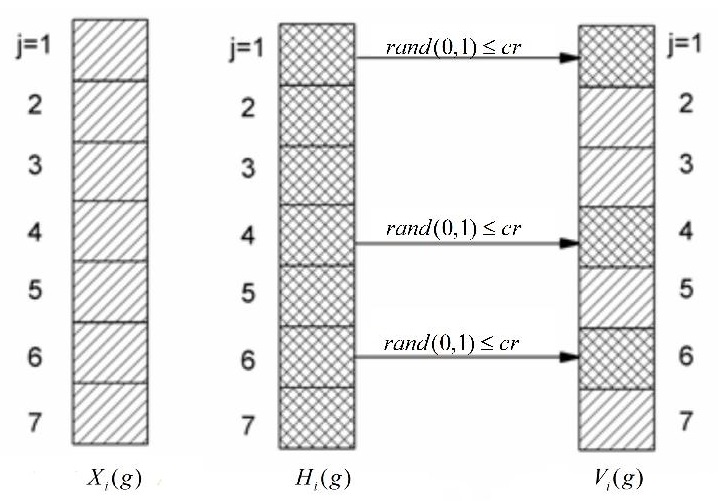
\includegraphics[width=6cm]{images/cross.png}
		\caption{交叉操作示意图}\label{fig2}
	\end{figurehere}
\item {选择}。选择操作在交叉操作之后进行,主要从原始个体$x_i^t$和变异个体$u_i^t$中选择出下一代个体$u_i^{t+1}$。
在标准差分进化算法中,利用一对一的贪心策略对下一代个体进行选择,具体选择策略如式5所示。其中,$f(x)$为个体
适应度计算函数。
	\begin{equation}
		\begin{split}
			x_i^t+1 =
			\begin{cases}
				u_i^t,\qquad \mathrm{if} \quad f(u_i^t)< f(x_i^t)\\
				t_i^t,\qquad else
			\end{cases}
		\end{split}
	\end{equation}
\end{enumerate}

\subsection{差分进化算法的其它形式}
\indent 上述所介绍的是最基本的差分进化算法,在实际的应用当中,基于基本的差分进化算法,发展出了几种不同的形式。
差分算法的不同种类以$DE/a/b$表示,其中,$a$表示变异个体的选择方式,$b$表示差向量的个数。上述的基本差分进化算法
可表示为$DE/rand/1$,表示算法变异个体的选择方式为随机选择,差向量的个数为1个。除此之外,还有以下几种差分进化算法。
\begin{enumerate}[fullwidth,itemindent=2em,label=(\arabic*)]
\item {\bf DE/best/1}。其变异操作如式6所示,在选择变异个体时,算法每次均选择种群内适应度最优的个体。在选择差向量时,
从当前种群中任意选择两个个体,得到一个差向量。
	\begin{equation}
		\begin{split}
			v_i^t = x_{best}^t+F\left(X_{p1}^t-X_{p2}^t\right)
		\end{split}
	\end{equation}

\item {\bf DE/current to best/1}。其变异操作如式7所示,在选择变异个体时,算法随机选择种群内一个个体。
在选择差向量时,一个差向量为当前种群最优个体与当前个体差向量,另一个差向量为种群随机选择两个个体的差向量。
	\begin{equation}
		\begin{split}
			v_i^t = x_{i}^t+F\left(x_{best}^t-x_{i}^t\right)+F\left(x_{p1}^t-x_{p2}^t\right)
		\end{split}
	\end{equation}

\item {\bf DE/best/2}。其变异操作如式8所示,在选择变异个体时,算法每次均选择种群内适应度最优的个体。
在选择差向量时,从当前种群随机选择四个不同个体,得到两个差向量。
	\begin{equation}
		\begin{split}
			v_i^t=x_{best}^t+F\left(x_{p1}^t-x_{p2}^t\right)+F\left(x_{p3}^t-x_{p4}^t\right)
		\end{split}
	\end{equation}

\item {\bf DE/rand/2。}其变异操作如式9所示,在选择变异个体时,算法随机选择种群内一个个体。
在选择差向量时,从当前种群随机选择四个不同个体,得到两个差向量。
	\begin{equation}
		\begin{split}
			v_i^t=x_{i}^t+F\left(x_{p1}^t-x_{p2}^t\right)+F\left(x_{p3}^t-x_{p4}^t\right)
		\end{split}
	\end{equation}
\end{enumerate}

\subsection{控制参数的选择}
\indent 控制参数对差分进化算法性能有很大的影响,以下介绍参数选取的一般规则。
\begin{enumerate}[fullwidth,itemindent=2em,label=(\arabic*)]
\item {种群数量}。假设问题解空间维数为$D$,则种群数量$M$取值一般在$5D\thicksim 10D$之间,另外,$M$的取值不能小于4,
否则,变异操作无法进行。

\item {变异算子}。变异算子$F$用于决定偏差向量的放大比例。$F$取值一般在$[0,2]$之间,通常取0.5,若种群过早
收敛,则应增加$F$的值。

\item {交叉算子}。交叉算子$cr$用于决定交叉染色体所占比例。$cr$的取值一般在$[0,1]$之间,较好的选择在0.3左右。
$cr$取值偏大,收敛速度加快,但易发生早熟现象。
\end{enumerate}

\indent 上述参数的选择策略仅仅针对一般情况,实际问题千变万化,参数的取值与目标函数的特性、收敛速度的要求
以及求解精度的要求都有关。在实际应用中,需要通过实验分析,结合上述规律,确定参数的合适取值。


\section{差分进化算法改进}
\subsection{参数自适应}
\indent 在标准差分进化算法中,变异算子$F$和交叉算子$cr$对算法的性能有较大的影响。基本的差分算法中,上述两个参数
一般取实常数。变异算子或交叉算子过大,算法搜索效率低下,求得的全局最优解的精度较低;变异算子或交叉算子过小,种群
多样性降低,易出现“早熟”现象。相比于标准的差分进化算法,参数自适应算法通过实时改变参数的数值,克服了以上缺点,大大
扩展了差分进化算法的应用范围。\\
\indent 针对变异算子$F$,在变异步骤,将随机选择的三个个体按照适应度进行从优到劣的排序,分别为$x_b^t$,$x_m^t$,
$x_w^t$,对应的适应度分别为$f_b$,$f_m$,$f_w$,变异个体的计算如式10所示。
	\begin{equation}
		\begin{split}
			v_i^t=x_{b}^t+F_i\left(x_{m}^t-x_{w}^t\right)
		\end{split}
	\end{equation}
$F_i$为自适应的变异算子,其取值根据差分向量两个个体的自适应度变化,以平衡全局搜索和局部搜索之间的矛盾。自适应变异
算子$F_i$的计算方法如式11所示,其中,$F_I$取值为0.1,$F_U$取值为0.9。
	\begin{equation}
		\begin{split}
			F_i = F_l +\left(F_u-F_l\right)\frac{f_m-f_b}{f_w-f_b}
		\end{split}
	\end{equation}
\indent 针对交叉算子$cr$,在算法迭代的过程中,对于适应度较好的解,取较小的$cr$,使得该解进入下一代的机会变大;
对于适应度较差的解,取较大的$cr$,加快改变该个体的结构,使该解被淘汰掉。$cr$的计算如式12所示。
	\begin{equation}
		\begin{split}
			cr_i =
			\begin{cases}
				cr_l+\left(cr_u-cr_l\right)\frac{f_i-f_{min}}{f_{max}-f_{min}}  \qquad \mathrm{if} \quad f_i>\bar{f} \\
				cr_l \qquad\qquad \qquad \qquad \qquad \quad \mathrm{if}\quad f_i<\bar{f}
			\end{cases}
		\end{split}
	\end{equation}
其中 $f_i$是个体$x_i$的适应度,$f_{min}$和$f_{max}$分别是当前种群中最差和最优个体的适应度,
$\bar{f}$是当前种群适应度平均值,$cr_l$和$cr_u$分别是$cr$的下限和上限,一般取$cr_l=0.1,cr_u=0.6$。

\subsection{并行差分进化算法}
\indent 并行处理可以极大提高差分进化算法的效率,扩展差分进化算法的应用领域。文献\supercite{7}研究了如何实现差分进化算法
的并行运算,以减少运算时间,提高运算性能。文中提出了一种并行计算模型,把群体进行分组,分配给不同的节点运行。研究表明,被
分配到不同计算节点的群体分组之间的信息交换程度对算法的性能产生了重要的影响。测试结果表明,相比于标准差分进化算法,并行
差分进化算法大大提高了计算性能。另外,文献\supercite{8}将并行差分进化算法应用到3D图像处理中,也获得了较好的效果。

\section{差分进化算法性能评估}
\indent 本章通过求解函数最优值的实例来对差分进化算法的性能进行分析与比较。要求解的函数表达式如式13所示,函数的图像如图2
所示。通过差分进化算法,求解该函数的最小值,在同样条件下(种群规模、迭代次数、搜素范围等),利用遗传算法对相同的问题进行求解。
	\begin{equation}
		\begin{split}
			f(x,y)=-20e^{-0.2\sqrt{\frac{x^2+y^2}{2}}}-e^{\frac{\cos2\pi x+\cos2\pi y}{2}}+20+e
		\end{split}
	\end{equation}
	
	\begin{figurehere}
		\centering
		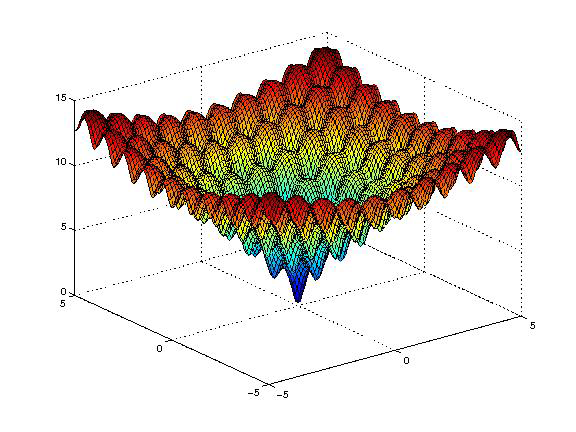
\includegraphics[width=6cm]{images/function.png}
		\caption{函数示意图}\label{fig2}
	\end{figurehere}
实验结果如图3和图4所示。其中,图3是利用遗传算法求解函数最小值的迭代过程,图4是利用标准差分进化算法求解函数最小值的
迭代过程。可以看出,相较于遗传算法,差分进化算法收敛更快。另外,在实验过程中,遗传算法表现并不稳定,每一次求解过程差别比较大,
相比之下,标准差分进化算法表现出更强的稳定性。


	\begin{figurehere}
		\centering
		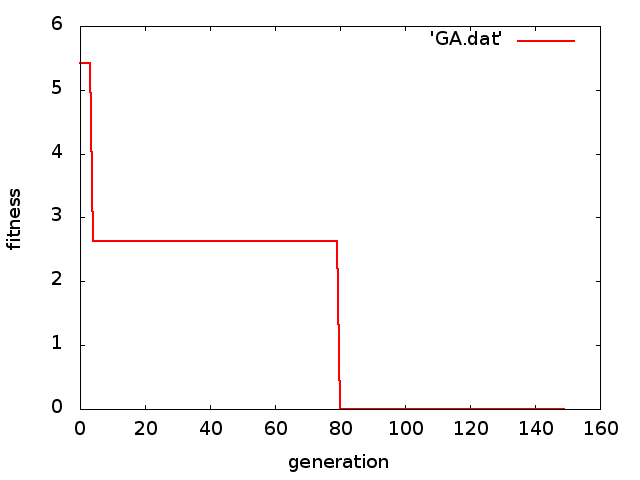
\includegraphics[width=6cm]{images/GA.png}
		\caption{遗传算法迭代过程示意图}\label{fig3}
	\end{figurehere}
	\begin{figurehere}
		\centering
		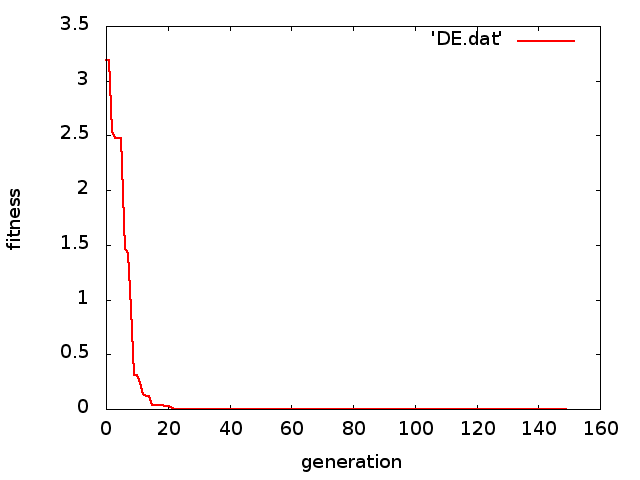
\includegraphics[width=6cm]{images/DE.png}
		\caption{差分进化算法迭代过程示意图}\label{fig4}
	\end{figurehere}

\section{结论}
\indent 本文重点介绍了差分进化算法的原理、框架、改进,在此基础上,通过实验,比较了差分进化算法与遗传算法的性能。
差分进化算法在非凸、多峰、非线性、连续不可微函数的优化问题上表现出极强的稳定性。另外,相比于遗传算法,差分进化算法
收敛速度更快。目前,差分进化算法已广泛应用于各个领域。但是,差分进化算法还有几点改进方向。
\begin{enumerate}[fullwidth,itemindent=2em,label=(\arabic*)]
\item 完善算法理论基础。相比于遗传算法,差分进化算法在收敛性、参数选取、算法鲁棒性等方面理论支持更少,进一步限制了其
应用范围。
\item 与其它算法的结合有待进一步研究。差分进化算法有自己独特的特点,因此,其适用范围有限。通过结合其它不同的算法,
对差分进化算法进行改进,可以提高差分进化算法的性能及其应用范围。
\end{enumerate}

%%%%%%%%%%%%%%%%%%%%%%%%%%%%%%%%%%%%%%%%%%%%%%%%%%%%%%%%%%%%%%%%
%  参考文献
%%%%%%%%%%%%%%%%%%%%%%%%%%%%%%%%%%%%%%%%%%%%%%%%%%%%%%%%%%%%%%%%
\small
\begin{thebibliography}{99}
\setlength{\parskip}{0pt}  %段落之间的竖直距离

\bibitem{1}Storn R, Price K. Differential evolution–a simple and efficient heuristic for global 
optimization over continuous spaces[J]. Journal of global optimization, 1997, 11(4): 341-359.
\bibitem{2}周艳平,顾幸生.差分进化算法研究进展[J].化工自动化及仪表,2007(03):1-6..
\bibitem{3}Liu B, Wang L, Jin Y, et al. Designing neural networks using hybrid particle swarm 
optimization[C]//International Symposium on Neural Networks. Springer, Berlin, Heidelberg, 2005: 391-397.
\bibitem{4}Kiranmai D, Jyothirmai A, Murty C V S. Determination of kinetic parameters in 
fixed-film bio-reactors: an inverse problem approach[J]. Biochemical engineering journal, 2005, 23(1): 73-83.
\bibitem{5}Aydin S, Temeltas H. Fuzzy-differential evolution algorithm for planning 
time-optimal trajectories of a unicycle mobile robot on a predefined path[J]. Advanced Robotics, 2004, 18(7): 725-748.
\bibitem{6}刘波,王凌,金以慧.差分进化算法研究进展[J].控制与决策,2007(07):721-729.
\bibitem{7}Tasoulis D K, Pavlidis N G, Plagianakos V P, et al. Parallel differential 
evolution[C]//Evolutionary Computation, 2004. CEC2004. Congress on. IEEE, 2004, 2: 2023-2029.
\bibitem{8}Salomon M, Perrin G R, Heitz F, et al. Parallel differential evolution: application 
to 3-d medical image registration[M]//Differential evolution. Springer, Berlin, Heidelberg, 2005: 353-411.

\end{thebibliography}
%%%%%%%%%%%%%%%%%%%%%%%%%%%%%%%%%%%%%%%%%%%%%%%%%%%%%%%%%%%%%%%%
%  分栏结束
%%%%%%%%%%%%%%%%%%%%%%%%%%%%%%%%%%%%%%%%%%%%%%%%%%%%%%%%%%%%%%%%
\end{multicols}
%%%%%%%%%%%%%%%%%%%%%%%%%%%%%%%%%%%%%%%%%%%%%%%%%%%%%%%%%%%%%%%%
%  文章结束
%%%%%%%%%%%%%%%%%%%%%%%%%%%%%%%%%%%%%%%%%%%%%%%%%%%%%%%%%%%%%%%%
\clearpage
\end{CJK*}
\end{document}
